%!TEX ROOT=../emnlp2023.tex

\section{Introduction}
\label{sec:introduction}
\todo{write}

% show figures/pipeline.png
\begin{figure}[h]
    \centering
    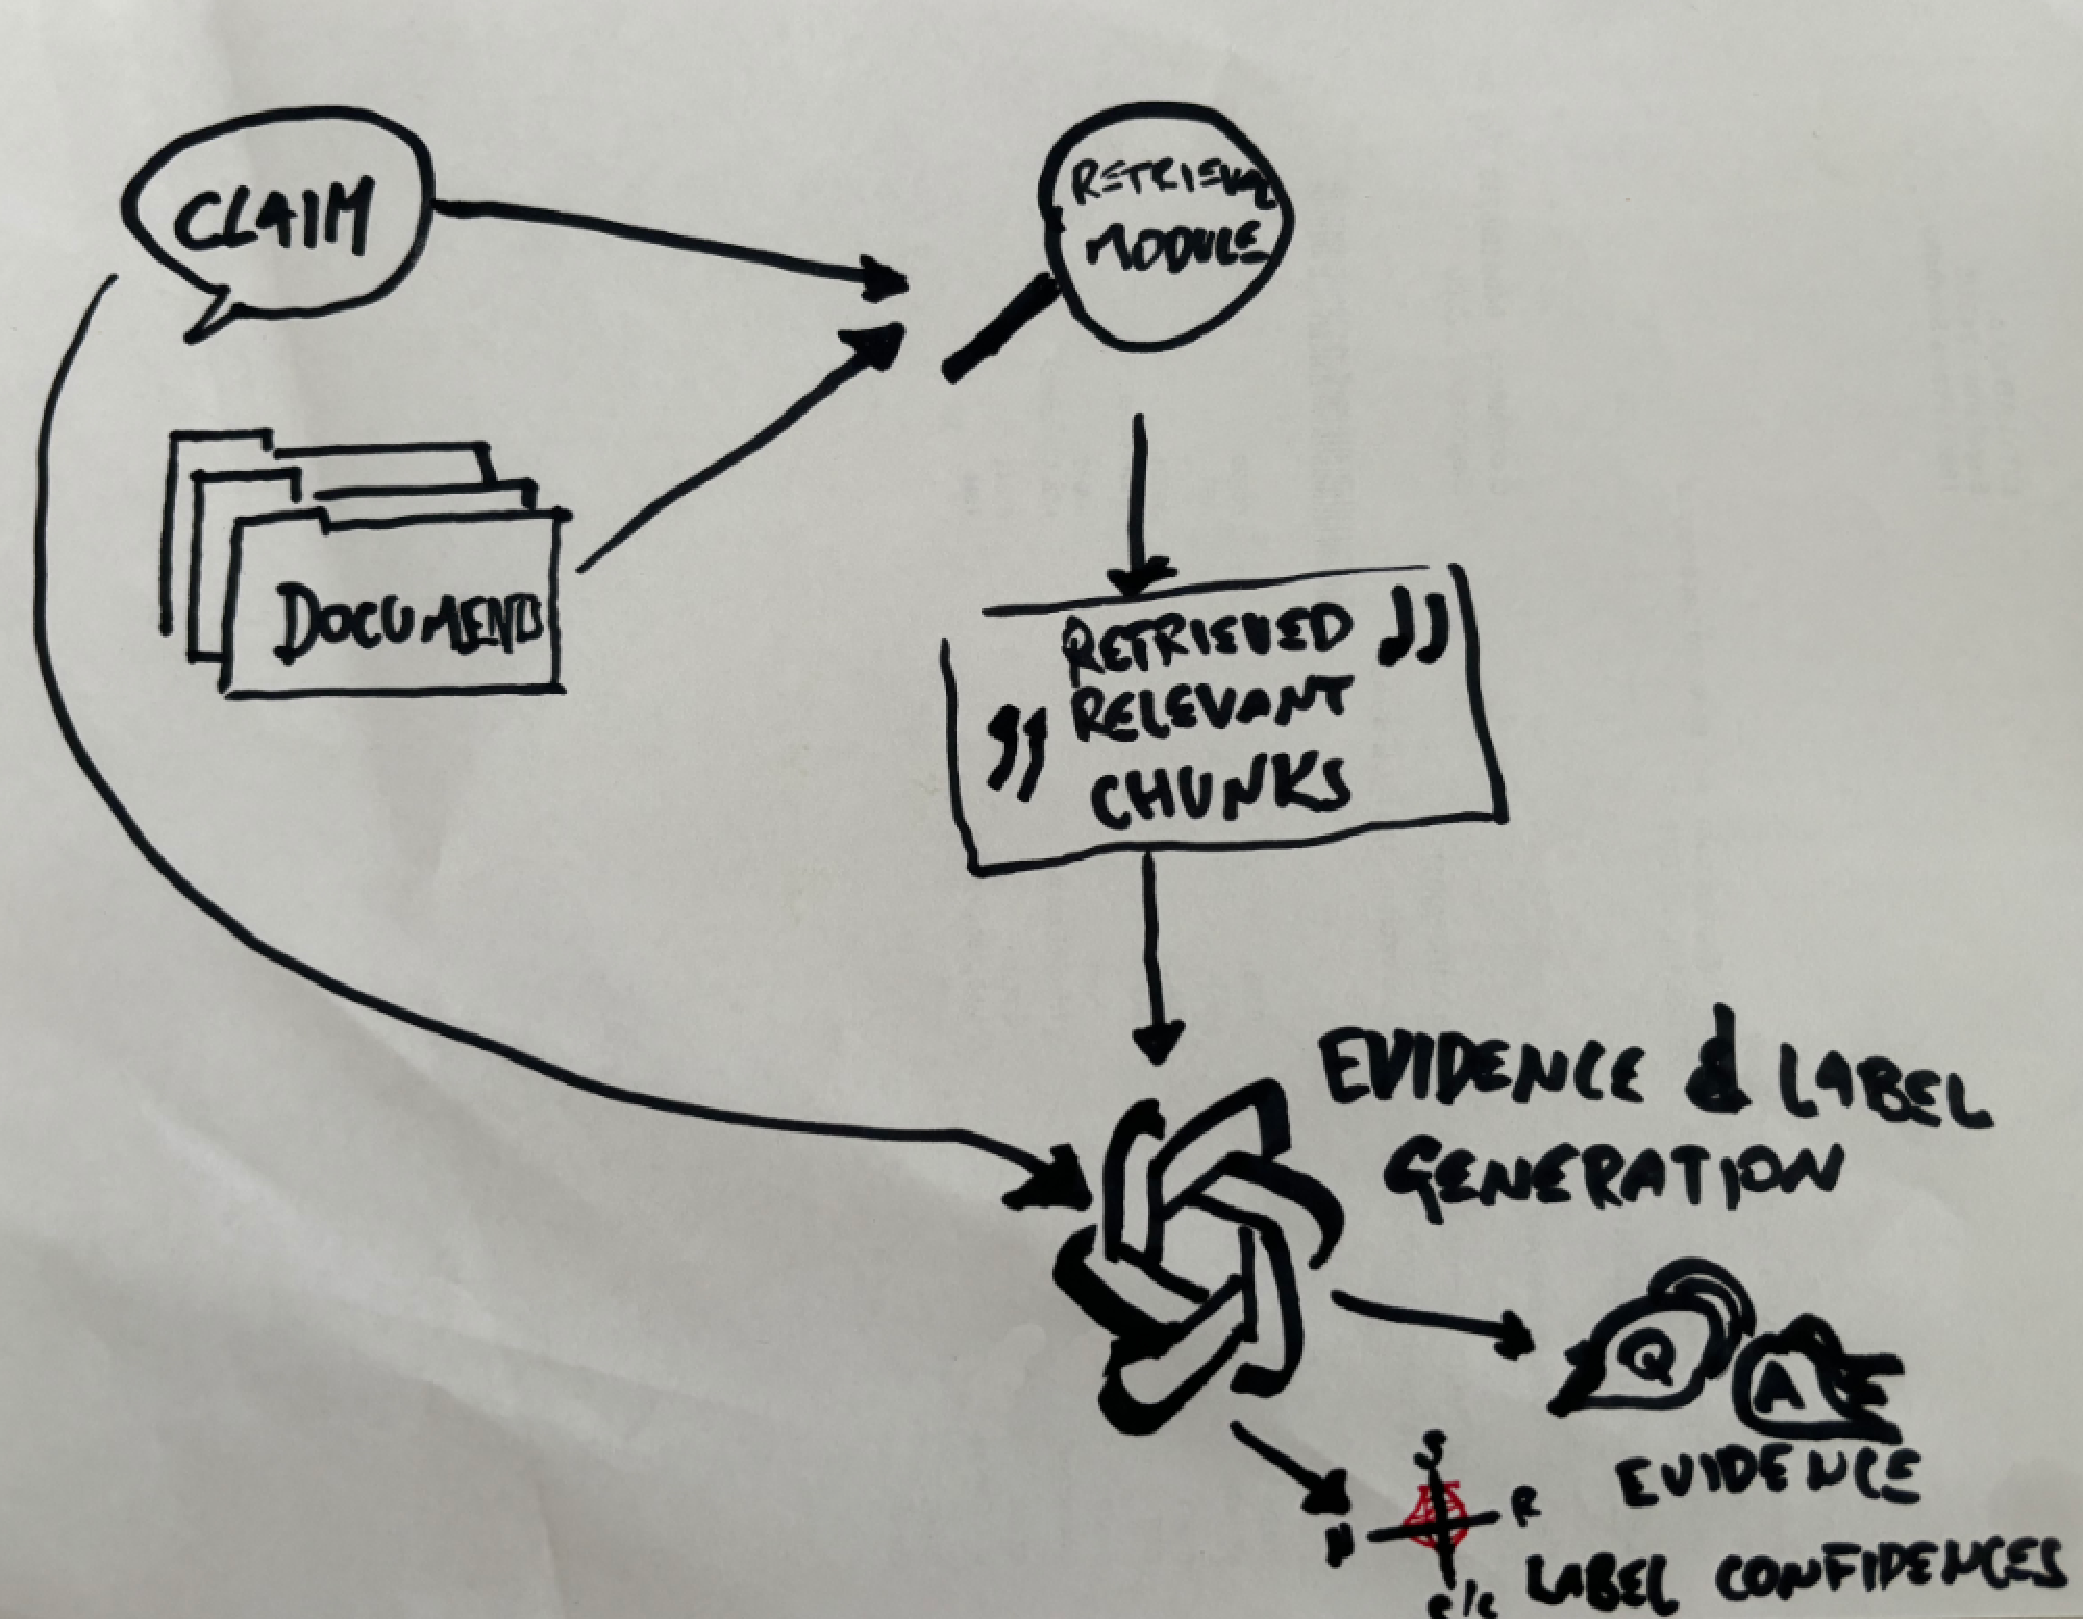
\includegraphics[width=0.47\textwidth]{figures/pipeline.pdf}
    \caption{Our pipeline}
    \label{fig:pipeline}
\end{figure}

\subsection{Related Work}
\label{sec:relwork}
\begin{enumerate}
    \item \textbf{\averitec{} score}~\cite{averitec2024} postulates method of unsupervised scoring of fact-checking pipeline against gold evidence and labels using Hungarian Meteor score and an accuracy metric
    \item \textbf{Baseline \averitec{} system} solves the task through 
    \item Our previous research on fact-checking pipelines~\cite{Ullrich2023,drchal2023pipelinedatasetgenerationautomated} using data similar to FEVER and \averitec{} shows significant superiority of fact-checking pipelines that retrieve the whole documents for the inference step, rather than out-of-context sentences
    \item \textbf{FEVER Shared Task}~\cite{thorne-etal-2018-fact} solutions such as Papelo~\cite{}
    \item \textbf{Retrieval-Augmented Generation (RAG) for Knowledge-Intensive Tasks}~\cite{rag} have demonstrated even simpler pipeline on the original FEVER dataset, 
\end{enumerate}

